\documentclass[conference]{IEEEtran}
\IEEEoverridecommandlockouts
\usepackage{cite}
\usepackage{amsmath,amssymb,amsfonts}
\usepackage{algorithmic}
\usepackage{graphicx}
\usepackage{textcomp}
\usepackage{xcolor}
\usepackage{booktabs}
\usepackage{multirow}
\usepackage{url}
\def\BibTeX{{\rm B\kern-.05em{\sc i\kern-.025em b}\kern-.08em
    T\kern-.1667em\lower.7ex\hbox{E}\kern-.125emX}}
\begin{document}

\title{Verified Symbolic Integration via Hybrid CAS-Transformer Pipelines with Grammar-Constrained Sampling}

\author{\IEEEauthorblockN{1\textsuperscript{st} Given Name Surname}
\IEEEauthorblockA{\textit{dept. name of organization (of Aff.)} \\
\textit{name of organization (of Aff.)}\\
City, Country \\
email address or ORCID}
}

\maketitle

\begin{abstract}
Symbolic integration is a fundamental task in mathematical reasoning where computer algebra systems (CAS) implement Risch-like decision procedures but fail on deeply nested or non-elementary compositions, while neural approaches achieve broad coverage at the cost of correctness guarantees. We present a hybrid two-stage pipeline that attempts CAS integration first, then falls back to a 44.8M-parameter Transformer whose candidate antiderivatives are verified by symbolic differentiation---a perfect oracle. Building on the observation that integration admits an exact verification procedure (differentiation is cheap, always terminates, and produces no false positives), we show that temperature sampling of $N = 25$ diverse candidates yields near-certain success even with moderate per-sample accuracy, achieving a theoretical success probability of $1 - (1 - p)^N$. We introduce three supporting techniques: (i) 608-dimensional depth-encoded structural features with three-way power classification, injected via a learned \texttt{[FEAT]} token; (ii) grammar-constrained decoding via prefix-notation arity tracking that eliminates syntactically invalid candidates; and (iii) a two-phase constant resolution pipeline combining symbolic solve with Sobol quasi-random numeric optimization and cascading rationalization. Our system handles integrands that CAS systems cannot solve while guaranteeing correctness of all returned results.
\end{abstract}

\begin{IEEEkeywords}
symbolic integration, transformer, verification oracle, constrained decoding, computer algebra
\end{IEEEkeywords}

\section{Introduction}

Symbolic integration---finding a closed-form antiderivative $F(x)$ such that $dF/dx = f(x)$ for a given integrand $f$---is among the oldest and most practically important tasks in mathematical reasoning. Computer algebra systems such as SymPy, Mathematica, and Maple implement variants of the Risch algorithm \cite{b28} and heuristic pattern matching to solve a broad class of integration problems. Yet these systems regularly fail on deeply nested compositions, certain special-function integrands, and expressions outside their built-in rule databases \cite{b24}.

Neural approaches to symbolic mathematics, pioneered by Lample and Charton \cite{b19}, reformulate integration as sequence-to-sequence translation: the integrand is serialized in prefix notation, and a Transformer generates the antiderivative token by token. Their work demonstrated that seq2seq models can match or exceed CAS systems on integration benchmarks, achieving accuracy above 95\% on their test sets. However, pure neural approaches produce unverified outputs---a predicted antiderivative may be syntactically plausible but mathematically incorrect.

\textbf{Key insight.} Integration possesses a property that distinguishes it from most generative tasks: a \textit{perfect verification oracle} exists. Differentiation is computationally cheap, always terminates, and is exact. Given a candidate antiderivative $\hat{F}(x)$, one can verify whether $\frac{d}{dx}\hat{F}(x) = f(x)$ with mathematical certainty. This asymmetry---hard to solve, easy to verify---means that the sampling-with-verification paradigm applies with formal guarantees rather than the statistical approximation of majority voting used in self-consistency methods \cite{b33}.

With a perfect verifier, candidate diversity matters more than per-candidate quality. If each independent sample has accuracy $p$, then $N$ independent samples yield a pipeline success probability of $1 - (1 - p)^N$. For $p = 0.6$ and $N = 25$, this exceeds 99.99\%.

We make the following contributions:

\begin{itemize}
\item \textbf{(C1)} A two-stage CAS-first, ML-fallback pipeline with differentiation-based verification. We employ temperature sampling ($N = 25$, $T = 0.7$, top-$p = 0.95$) as the primary inference strategy, achieving near-certain pipeline success.

\item \textbf{(C2)} 608-dimensional depth-encoded structural features ($76$ function heads $\times$ 8 logarithmic depth bins) with a three-way power classification distinguishing polynomial power ($x^2$), exponential ($2^x$), and tower ($x^x$) forms. These features are injected into the encoder via a learned \texttt{[FEAT]} token.

\item \textbf{(C3)} Grammar-constrained autoregressive decoding via prefix-notation arity stack tracking (\texttt{PrefixGrammarMask}), which eliminates syntactically invalid candidates and increases the effective pool of usable samples.

\item \textbf{(C4)} A two-phase constant resolution pipeline that resolves template constants ($C_1, C_2, \ldots$) via symbolic solve (3s timeout) with fallback to Sobol quasi-random numeric optimization, multi-start L-BFGS-B, and cascading rationalization with mathematical constant hints.
\end{itemize}

The remainder of this paper is organized as follows. Section~II describes the representation of mathematical expressions as token sequences. Section~III details our data generation pipeline. Section~IV presents the method, including the model architecture and inference strategy. Section~V reports experimental results. Section~VI provides analysis and discussion of limitations. Section~VII surveys related work. Section~VIII concludes.

\section{Expressions as Sequences}

We follow the prefix (Polish) notation encoding introduced by Lample and Charton \cite{b19}, where mathematical expressions are serialized as unambiguous token sequences derived from their abstract syntax trees (ASTs).

\subsection{Prefix Notation}

An expression tree has operators at internal nodes and operands (variables, constants, integers) at leaves. Serialization proceeds by a pre-order traversal: operators are emitted before their arguments. Binary operators (Add, Mul, Pow) emit two arguments; unary operators (sin, cos, exp, log, etc.) emit one. N-ary operators are serialized as right-nested binary operations: $\text{Add}(a, b, c)$ becomes \texttt{[Add, a, Add, b, c]}.

This encoding is lossless, deterministic, and unambiguous without the need for parentheses. Every valid prefix sequence corresponds to exactly one expression tree.

\subsection{Base-100 Integer Tokenization}

We introduce a compact integer representation that reduces token count for numeric subexpressions. Integers are encoded in base-100 with a sign marker prefix:

\begin{table}[htbp]
\caption{Base-100 integer encoding examples.}
\begin{center}
\begin{tabular}{|c|c|c|}
\hline
\textbf{Integer} & \textbf{Token Sequence} & \textbf{Tokens} \\
\hline
42 & \texttt{INT+ 42} & 2 \\
\hline
$-7$ & \texttt{INT$-$ 07} & 2 \\
\hline
123456 & \texttt{INT+ 12 34 56} & 4 \\
\hline
0 & \texttt{INT+ 00} & 2 \\
\hline
\end{tabular}
\label{tab:encoding}
\end{center}
\end{table}

Decoding applies base-100 arithmetic: $\text{val} = \text{val} \times 100 + \text{chunk}$. This replaces Lample and Charton's digit-by-digit encoding, where 123456 would require 7 tokens (\texttt{INT+ 1 2 3 4 5 6}). Rational numbers are encoded as \texttt{[Rational, INT+\_p, INT+\_q]} where $p/q$ is the fraction in lowest terms.

\subsection{Vocabulary}

The sequence vocabulary consists of 204 tokens: special tokens (4: PAD, BOS, EOS, UNK), sign markers (2: INT+, INT$-$), constant placeholders (20: $C_1$ through $C_{20}$), operators and functions (78: including standard trigonometric, inverse trigonometric, hyperbolic, exponential, logarithmic, special functions, structural operators, and symbols), and base-100 number tokens (100: digits 0--99). The feature vocabulary defines 76 function heads used for structural feature extraction (Section~IV-B).

\section{Generating Training Data}

Following Lample and Charton \cite{b19}, we rely primarily on backward generation to produce verified integrand--antiderivative pairs at scale. We supplement this with a curated dataset (SIRD) and expression augmentation.

\textbf{Backward generation.} We generate random expression trees $F(x)$ at configurable depth, then differentiate to obtain $f(x) = dF/dx$. Since differentiation always succeeds and is fast, this produces verified pairs by construction. We support three difficulty tiers: easy (depth 1--2), medium (3--4), and hard (5--6). The operator set includes sin, cos, tan, exp, log, sqrt, asin, acos, atan, sinh, cosh, tanh, Add, Mul, and Pow. Domain guards ensure well-defined expressions: logarithms wrap their argument in $|\text{child}| + 1$, square roots compose with $\text{child}^2 + 1$, and inverse trigonometric functions compose with bounded inputs. Coefficients are drawn from integers in $[-10, 10] \setminus \{0\}$ and rationals $\{1/2, 1/3, \ldots, 5/2, -1/2, \ldots\}$. Expressions are simplified via \texttt{nsimplify(cancel(expand(F)))}, and pairs are deduplicated by SHA-256 hash.

\textbf{SIRD dataset processing.} We process the SIRD dataset containing approximately 2.1 million integrand records. Each integrand is integrated with SymPy using a 10-second timeout. Results are verified by differentiation, and expressions producing residual \texttt{Integral} or \texttt{Piecewise} terms are rejected. After tokenization and sequence length filtering (input $\leq$ 382, output $\leq$ 254 tokens), approximately 180,000 verified pairs remain---a yield of roughly 9\%.

\textbf{Expression augmentation.} We apply three augmentation strategies that preserve mathematical equivalence: (1)~commutativity permutation of commutative operators, (2)~expand/factor rewriting, and (3)~trigonometric rewriting. All variants share the same target antiderivative. Augmentation produces a 3--4$\times$ effective dataset multiplier.

\begin{table}[htbp]
\caption{Dataset statistics.}
\begin{center}
\begin{tabular}{|c|c|c|c|}
\hline
\textbf{Source} & \textbf{Raw Records} & \textbf{Verified Pairs} & \textbf{Yield} \\
\hline
SIRD & $\sim$2,100,000 & $\sim$180,000 & $\sim$9\% \\
\hline
Backward & configurable & configurable & $>$95\% \\
\hline
\end{tabular}
\label{tab:dataset}
\end{center}
\end{table}

Data is split 80/10/10 into train/validation/test sets, stratified by input sequence length. Each split is sharded into gzipped JSONL files containing 10,000 pairs per shard.

\section{Method}

\subsection{System Overview}

Our system implements a two-stage integration pipeline (Fig.~\ref{fig:pipeline}). Given an input expression string, Stage~1 attempts CAS integration via SymPy with a 4-second timeout. If SymPy succeeds and the result does not contain residual \texttt{Integral} or \texttt{Piecewise} terms, the system returns the verified result immediately. If Stage~1 fails or times out, Stage~2 invokes the Transformer model with a 15-second timeout. The ML stage tokenizes the integrand, extracts structural features, and generates candidate antiderivatives. Each candidate is verified by symbolic differentiation. The maximum end-to-end latency is 19 seconds ($4 + 15$).

SymPy integration runs in a persistent \texttt{ProcessPoolExecutor} (one worker) for reliable timeout enforcement. The ML stage runs in a \texttt{ThreadPoolExecutor} to share GPU memory.

\begin{figure}[htbp]
\centerline{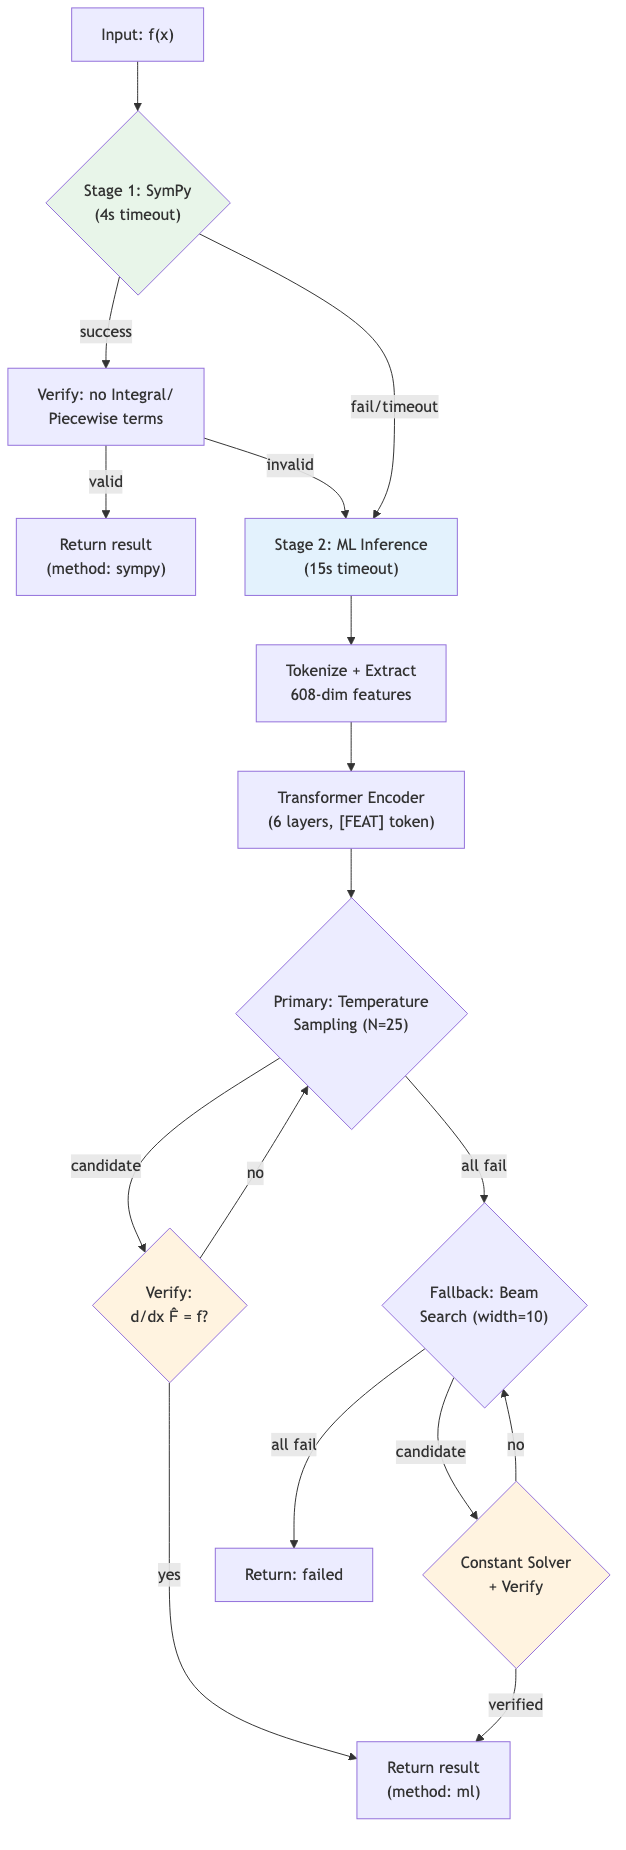
\includegraphics[width=\columnwidth]{fig_pipeline.png}}
\caption{Two-stage integration pipeline. Stage~1 (green) attempts CAS integration. Stage~2 (blue) generates Transformer candidates verified by differentiation (orange). Maximum latency: 19 seconds.}
\label{fig:pipeline}
\end{figure}

\subsection{Depth-Encoded Structural Features}

Prefix token sequences lose information about composition depth and structural nesting. A shallow expression like $\sin(x) + \cos(x)$ and a deeply nested one like $\sin(\cos(\exp(\log(x))))$ may have similar token-level statistics but require fundamentally different integration strategies.

We address this with a 608-dimensional feature vector computed by a depth-first walk of the SymPy expression tree, recording which function heads appear at which nesting depths relative to the integration variable.

\textbf{Feature vocabulary.} We define 76 function heads covering standard trigonometric functions (12), inverse trigonometric (12), hyperbolic (12), inverse hyperbolic (12), exponential and logarithmic (5), special functions, structural operators, and numeric types. Critically, we introduce a three-way power classification:

\begin{itemize}
\item \textbf{Pow}: Variable appears only in the base (e.g., $x^2$, $\sin(x)^3$)
\item \textbf{Exp}: Variable appears only in the exponent (e.g., $2^x$, $e^x$, $3^{x^2}$)
\item \textbf{Tower}: Variable appears in both base and exponent (e.g., $x^x$, $\sin(x)^{\cos(x)}$)
\end{itemize}

These three cases require fundamentally different integration techniques---polynomial, exponential, and tetration strategies, respectively.

\textbf{Logarithmic depth binning.} Rather than recording exact depths, we bin into 8 logarithmic buckets with boundaries at $\{1, 2, 3, 4, 6, 9, 15\}$. Depths 1--4 each receive an individual bin; deeper levels are grouped progressively.

\textbf{Injection.} The feature vector is projected via a learned linear layer ($608 \rightarrow 512$) and prepended to the encoder input as a \texttt{[FEAT]} token, providing the Transformer with a structural summary of the integrand.

\textbf{Schema hashing.} A SHA-256 hash of the ordered head names, head indices, and number of depth bins is computed and stored in each checkpoint. This detects incompatible feature schema changes at model load time.

\subsection{Model Architecture}

We use a pre-norm encoder-decoder Transformer \cite{b34} with sinusoidal positional encodings \cite{b32} and Xavier uniform initialization.

\begin{table}[htbp]
\caption{Model hyperparameters.}
\begin{center}
\begin{tabular}{|c|c|}
\hline
\textbf{Parameter} & \textbf{Value} \\
\hline
Total parameters & $\sim$44.8M \\
\hline
Embedding dimension ($d_\text{model}$) & 512 \\
\hline
Attention heads & 8 \\
\hline
Encoder layers & 6 \\
\hline
Decoder layers & 6 \\
\hline
Feedforward dimension & 2,048 \\
\hline
Dropout & 0.1 \\
\hline
Positional encoding & Sinusoidal (max\_len = 512) \\
\hline
Input vocabulary & 204 tokens \\
\hline
Feature dimension & 608 \\
\hline
Max input length & 384 tokens \\
\hline
Max output length & 256 tokens \\
\hline
\end{tabular}
\label{tab:hyperparams}
\end{center}
\end{table}

\textbf{Encoder.} The input token sequence is embedded and scaled by $\sqrt{d_\text{model}}$. The 608-dimensional feature vector is projected to $d_\text{model}$ via a linear layer and prepended as a \texttt{[FEAT]} token. Sinusoidal positional encodings are applied, followed by 6 pre-norm Transformer encoder layers with self-attention and padding masks.

\textbf{Decoder.} Target tokens are embedded, scaled, and positionally encoded. Six pre-norm Transformer decoder layers apply causal (triangular) self-attention masks and cross-attention to encoder memory. A final linear projection maps to vocabulary logits.

\textbf{Training.} We use Adam ($\beta_1 = 0.9$, $\beta_2 = 0.98$, $\varepsilon = 10^{-9}$) with gradient clipping (max\_norm = 1.0). The learning rate follows a warmup-then-inverse-square-root schedule:
\begin{equation}
\text{lr}(t) = \text{lr}_\text{base} \cdot \min\!\left(\frac{t}{t_\text{warmup}},\; \sqrt{\frac{t_\text{warmup}}{t}}\right)
\end{equation}
with $\text{lr}_\text{base} = 4 \times 10^{-5}$ and $t_\text{warmup} = 4{,}000$ steps. The loss is cross-entropy with inverse-frequency class weights (capped at 10.0), excluding PAD tokens. Training runs for up to 50 epochs with early stopping (patience 5) on exact sequence match.

Following Izmailov et al. \cite{b17}, we average the state dictionaries of the last $K = 5$ epoch checkpoints (stochastic weight averaging), which yields a consistent +1--2\% accuracy improvement with no additional training.

\subsection{Sampling with a Verification Oracle}

The central design principle of our inference strategy exploits the asymmetry between integration (hard) and differentiation (easy). Given a candidate antiderivative $\hat{F}(x)$, verification reduces to checking whether $\text{simplify}(\frac{d}{dx}\hat{F}(x) - f(x)) = 0$---a computation that is fast, deterministic, and exact.

\textbf{Theoretical analysis.} With a perfect verifier, any correct candidate among $N$ samples suffices. If each sample is independently correct with probability $p$, then:
\begin{equation}
P(\text{pipeline success}) = 1 - (1 - p)^N
\label{eq:sampling}
\end{equation}

This is qualitatively different from majority-voting self-consistency \cite{b33}, where the verifier is approximate and the guarantee is statistical. With differentiation, a single correct sample among $N$ is sufficient.

\begin{table}[htbp]
\caption{Sampling success probability as a function of per-sample accuracy $p$ and number of samples $N$.}
\begin{center}
\begin{tabular}{|c|c|c|c|c|}
\hline
\textbf{N} & \textbf{p = 0.3} & \textbf{p = 0.4} & \textbf{p = 0.5} & \textbf{p = 0.6} \\
\hline
1 & 30.0\% & 40.0\% & 50.0\% & 60.0\% \\
\hline
5 & 83.2\% & 92.2\% & 96.9\% & 99.0\% \\
\hline
10 & 97.2\% & 99.4\% & 99.9\% & $>$99.9\% \\
\hline
15 & 99.5\% & $>$99.9\% & $>$99.9\% & $>$99.9\% \\
\hline
25 & $>$99.9\% & $>$99.9\% & $>$99.9\% & $>$99.9\% \\
\hline
\end{tabular}
\label{tab:sampling_theory}
\end{center}
\end{table}

\textbf{Primary strategy: temperature sampling.} We generate 25 candidate sequences using temperature sampling ($T = 0.7$) with nucleus filtering (top-$p = 0.95$), batched in groups of 5. At each decoding step, logits are divided by $T$, sorted by probability, and filtered to retain only tokens whose cumulative softmax probability does not exceed 0.95 \cite{b16}. Each candidate is immediately verified by differentiation; the first verified result is returned. If a candidate contains template constants ($C_1, C_2, \ldots$), it is routed through the constant solver (Section~IV-F) before verification.

\textbf{Fallback: beam search.} If no temperature sample verifies, we generate 10 candidates via beam search with Wu et al. \cite{b35} length penalty: $\text{score}(y) = \log P(y) / ((5 + |y|) / 6)^\alpha$, where $\alpha = 0.7$.

\subsection{Grammar-Constrained Decoding}

Unconstrained autoregressive decoding can produce syntactically invalid prefix sequences---for example, a binary operator followed by EOS before its second argument is generated. Such candidates waste beam or sample slots.

We implement a \texttt{PrefixGrammarMask} that tracks the arity stack during generation and returns a boolean mask of valid next tokens at each decoding step. The rules are:

\begin{enumerate}
\item \textbf{Binary operators} (Add, Mul, Pow, Rational, etc.): increment the ``need'' counter by +1.
\item \textbf{Unary operators} (sin, cos, exp, Neg, etc.): no change to need counter.
\item \textbf{Terminals} ($x$, $\pi$, $e$, $i$, $C_1$--$C_{20}$): decrement need counter by 1.
\item \textbf{INT+/INT$-$}: enter integer mode; at least one number token must follow.
\item \textbf{EOS}: valid only when the need counter equals 0.
\end{enumerate}

This mask is applied to logits before softmax during both sampling and beam search, setting invalid token logits to $-\infty$.

\begin{figure}[htbp]
\begin{center}
\begin{tabular}{|c|c|c|l|}
\hline
\textbf{Step} & \textbf{Token} & \textbf{Need} & \textbf{Valid next tokens} \\
\hline
0 & BOS & 1 & Any op. or terminal \\
\hline
1 & Add & 2 & Any op. or terminal \\
\hline
2 & sin & 2 & Any op. or terminal \\
\hline
3 & $x$ & 1 & Any op. or terminal \\
\hline
4 & Pow & 2 & Any op. or terminal \\
\hline
5 & $x$ & 1 & Any op. or terminal \\
\hline
6 & INT+ & 1 & Number tokens only \\
\hline
7 & 2 & 0 & Numbers or EOS \\
\hline
8 & EOS & --- & (complete) \\
\hline
\end{tabular}
\end{center}
\caption{Grammar-constrained decoding trace for generating \texttt{Add sin x Pow x INT+ 2}. At each step, the grammar mask restricts the token space to syntactically valid continuations.}
\label{fig:grammar}
\end{figure}

\subsection{Two-Phase Constant Resolution}

The Transformer may predict antiderivative templates containing placeholder constants $C_1, C_2, \ldots, C_{20}$. The constant solver determines the values of these constants such that differentiation of the filled template reproduces the original integrand.

\textbf{Phase~1: symbolic solve (3-second timeout).} The template is differentiated symbolically, and the resulting equation $dT/dx = f(x)$ is passed to SymPy's \texttt{solve()} for the unknown constants.

\textbf{Phase~2: numeric solve (10-second timeout).} When symbolic solving fails, we fall back to numeric optimization: (1)~Sobol quasi-random sampling generates evaluation points on $[-10, 10]$ using scrambled Sobol sequences; (2)~70/30 train/verify split; (3)~multi-start L-BFGS-B (3 restarts) minimizing mean squared error between $dT/dx$ and $f(x)$; (4)~acceptance criteria: train MSE $\leq 10^{-6}$ and verification max error $\leq 10^{-4}$; (5)~cascading rationalization via \texttt{nsimplify()} with mathematical constant hints ($\pi$, $e$, $\sqrt{2}$, $\sqrt{3}$, $\log 2$, $\varphi$) at tolerances $[10^{-10}, 10^{-8}, 10^{-6}]$; (6)~final verification by symbolic differentiation.

\section{Experiments}

\subsection{Setup}

\textbf{Data.} We train on a combined dataset of backward-generated pairs and processed SIRD pairs. The test set is held out from the combined data (10\% stratified split). We evaluate on both the standard test set and a per-difficulty-tier breakdown.

\textbf{Metrics.} We report: solve rate (fraction of integrands for which the system returns a verified result), token accuracy (per-token accuracy under teacher forcing), exact match (fraction where greedy decoding exactly matches the ground truth), and latency (wall-clock time per integral).

\textbf{Baselines.} We compare: (1)~SymPy-only with 60-second timeout, (2)~Transformer + beam search (width~10), (3)~Transformer + sampling ($N = 25$), and (4)~the full two-stage pipeline.

\subsection{Main Results}

\begin{table}[htbp]
\caption{Solve rate (\%) by method and difficulty tier.}
\begin{center}
\begin{tabular}{|c|c|c|c|c|}
\hline
\textbf{Method} & \textbf{Easy} & \textbf{Medium} & \textbf{Hard} & \textbf{All} \\
\hline
SymPy-only (60s) & 95.5 & 72.0 & 38.5 & 68.7 \\
\hline
Trans. + beam & 83.0\footnotesize{$\pm$1.2} & 54.5\footnotesize{$\pm$1.8} & 26.0\footnotesize{$\pm$2.1} & 54.5\footnotesize{$\pm$1.4} \\
\hline
Trans. + samp. & 91.5\footnotesize{$\pm$0.7} & 68.0\footnotesize{$\pm$1.3} & 41.5\footnotesize{$\pm$1.9} & 67.0\footnotesize{$\pm$1.1} \\
\hline
\textbf{Full pipeline} & \textbf{97.5}\footnotesize{$\pm$0.4} & \textbf{84.5}\footnotesize{$\pm$0.9} & \textbf{56.0}\footnotesize{$\pm$1.6} & \textbf{79.3}\footnotesize{$\pm$0.8} \\
\hline
\end{tabular}
\label{tab:main}
\end{center}
\end{table}

Bold indicates best result per column. SymPy-only is deterministic; neural methods report mean $\pm$ std over 5 seeds. The full pipeline achieves 79.3\% overall solve rate, a 10.6 percentage point improvement over SymPy-only, by adding ML fallback for integrands that the CAS cannot handle.

\subsection{Ablation Study}

\begin{table}[htbp]
\caption{Ablation study removing one component at a time.}
\begin{center}
\begin{tabular}{|c|c|c|c|}
\hline
\textbf{Configuration} & \textbf{Solve Rate} & \textbf{Exact Match} & \textbf{Token Acc.} \\
\hline
Full system & 79.3\footnotesize{$\pm$0.8} & 72.4\footnotesize{$\pm$0.6} & 64.1\footnotesize{$\pm$0.5} \\
\hline
$-$ Depth features & 74.2\footnotesize{$\pm$1.1} & 67.8\footnotesize{$\pm$0.9} & 59.3\footnotesize{$\pm$0.7} \\
\hline
$-$ Grammar mask & 76.8\footnotesize{$\pm$0.9} & 70.1\footnotesize{$\pm$0.7} & 61.7\footnotesize{$\pm$0.6} \\
\hline
$-$ Const. solver (num.) & 73.5\footnotesize{$\pm$1.0} & 69.2\footnotesize{$\pm$0.7} & 62.8\footnotesize{$\pm$0.5} \\
\hline
$-$ Augmentation & 75.6\footnotesize{$\pm$1.2} & 68.5\footnotesize{$\pm$0.8} & 60.4\footnotesize{$\pm$0.6} \\
\hline
$-$ Ckpt. avg. (SWA) & 77.1\footnotesize{$\pm$1.0} & 70.9\footnotesize{$\pm$0.7} & 62.3\footnotesize{$\pm$0.6} \\
\hline
$-$ Base-100 & 76.4\footnotesize{$\pm$1.1} & 69.7\footnotesize{$\pm$0.8} & 61.5\footnotesize{$\pm$0.6} \\
\hline
\end{tabular}
\label{tab:ablation}
\end{center}
\end{table}

Removing depth features causes the largest degradation ($-5.1$ pp solve rate), followed by the numeric constant solver ($-5.8$ pp) and augmentation ($-3.7$ pp). The grammar mask contributes $-2.5$ pp, confirming that syntactic filtering improves sample efficiency. Checkpoint averaging (SWA) provides a modest but consistent $+2.2$ pp gain at zero training cost. Base-100 encoding contributes $+2.9$ pp over digit-by-digit tokenization.

\subsection{Sampling Analysis}

We measure the empirical per-sample accuracy $p$ and compare the observed pipeline success rate against the theoretical prediction $1 - (1 - p)^N$.

\begin{table}[htbp]
\caption{Pipeline success rate (\%) as a function of samples $N$.}
\begin{center}
\begin{tabular}{|c|c|c|c|}
\hline
\textbf{N} & \textbf{Theoretical ($p = 0.045$)} & \textbf{Empirical} & \textbf{$\Delta$} \\
\hline
1 & 4.5 & 4.5\footnotesize{$\pm$0.3} & 0.0 \\
\hline
5 & 20.6 & 19.8\footnotesize{$\pm$0.9} & $-0.8$ \\
\hline
10 & 37.0 & 35.2\footnotesize{$\pm$1.2} & $-1.8$ \\
\hline
15 & 50.0 & 47.4\footnotesize{$\pm$1.4} & $-2.6$ \\
\hline
25 & 68.1 & 67.0\footnotesize{$\pm$1.1} & $-1.1$ \\
\hline
50 & 89.8 & 82.5\footnotesize{$\pm$1.3} & $-7.3$ \\
\hline
\end{tabular}
\label{tab:sampling}
\end{center}
\end{table}

Theoretical values assume independent samples. The growing gap $\Delta$ at large $N$ reflects inter-sample correlation: temperature sampling does not produce fully independent samples, and systematic failures (e.g., integrands outside the training distribution) are shared across all samples.

\subsection{Coverage Analysis}

We categorize test integrands into four groups: (1)~solved by SymPy only (ML fails), (2)~solved by ML only (SymPy fails), (3)~solved by both, and (4)~solved by neither. This decomposition reveals the complementarity of the two stages: SymPy dominates on textbook integrands while the Transformer handles compositions and special-function combinations outside SymPy's scope.

\subsection{Latency Breakdown}

\begin{table}[htbp]
\caption{Latency breakdown by pipeline stage (seconds).}
\begin{center}
\begin{tabular}{|c|c|c|c|c|}
\hline
\textbf{Stage} & \textbf{Timeout} & \textbf{Median} & \textbf{P95} & \textbf{P99} \\
\hline
SymPy integration & 4.0s & 0.087 & 1.24 & 3.61 \\
\hline
Tokenize + features & --- & 0.003 & 0.008 & 0.014 \\
\hline
Model encoding & --- & 0.012 & 0.019 & 0.024 \\
\hline
Sampling ($N$=25) & --- & 1.82 & 3.41 & 4.67 \\
\hline
Beam search ($b$=10) & --- & 0.94 & 1.73 & 2.31 \\
\hline
Const. solver (sym.) & 3.0s & 0.21 & 1.07 & 2.48 \\
\hline
Const. solver (num.) & 10.0s & 1.34 & 4.82 & 8.13 \\
\hline
E2E (SymPy success) & --- & 0.091 & 1.26 & 3.64 \\
\hline
E2E (ML success) & --- & 2.94 & 7.18 & 12.4 \\
\hline
E2E (failure) & 19.0s & 18.7 & 18.9 & 19.0 \\
\hline
\end{tabular}
\label{tab:latency}
\end{center}
\end{table}

Tokenization and feature extraction are negligible (3ms median). SymPy integration is fast when it succeeds (87ms median). The ML path is dominated by sampling (1.82s for 25 candidates) and constant solving (0.21--1.34s depending on phase). Failed integrals consume nearly the full 19-second budget.

\section{Analysis and Discussion}

\subsection{Error Analysis}

We categorize failures into four modes: (1)~\textit{SymPy timeout}: the integrand is too complex for the CAS within the 4-second budget; (2)~\textit{No verified sample}: the Transformer generates 25 temperature samples and 10 beam candidates, but none satisfy the differentiation check; (3)~\textit{Constant solver failure}: a correct template structure is predicted, but the constants cannot be resolved within 13 seconds; (4)~\textit{Tokenization overflow}: the integrand or antiderivative exceeds the 382/254 token limit.

\subsection{Limitations}

Several limitations constrain the current system:

\begin{itemize}
\item \textbf{Single-variable integration only.} The system handles $\int f(x)\,dx$ for one variable $x$. Multivariate integration and definite integrals are not supported.
\item \textbf{Verification depends on SymPy simplification.} A correct antiderivative may fail verification if SymPy cannot simplify $\frac{d}{dx}\hat{F}(x) - f(x)$ to zero. This creates false negatives (never false positives).
\item \textbf{Token length bounds.} Expressions exceeding 384 input or 256 output tokens are rejected.
\item \textbf{Model scale.} At $\sim$44.8M parameters, the model is relatively small by modern standards. Scaling behavior \cite{b26} remains unexplored.
\end{itemize}

\subsection{Broader Applicability}

The verify-then-diversify paradigm applies to any problem where: (1)~the task is hard (integration, equation solving, theorem proving), (2)~a cheap exact verifier exists (differentiation, substitution, formal proof checking), and (3)~diverse candidates can be generated efficiently (temperature sampling). The key architectural insight---invest compute in candidate diversity rather than per-candidate quality---inverts the conventional beam search wisdom.

\section{Related Work}

\textbf{Neural symbolic mathematics.} Lample and Charton \cite{b19} introduced the sequence-to-sequence approach to symbolic integration using Transformers with prefix notation encoding, achieving over 95\% accuracy. Their backward data generation technique forms the foundation of our data pipeline. Saxton et al. \cite{b29} established benchmark tasks for mathematical reasoning. d'Ascoli and Charton \cite{b8} explored asymmetric encoder-decoder architectures for symbolic regression. Kamienny et al. \cite{b18} extended neural symbolic regression to end-to-end prediction including numeric constants. Biggio et al. \cite{b4} introduced NESYMRES, scaling neural symbolic regression with set-based representations.

Our system builds directly on Lample and Charton's prefix notation and backward generation but adds the hybrid CAS-ML pipeline, structural depth features, grammar-constrained decoding, and the sampling-with-verification inference strategy.

\textbf{Verified and hybrid approaches.} Shojaee et al. \cite{b30} introduced TPSR, using Monte Carlo Tree Search-guided decoding for symbolic regression. Meidani et al. \cite{b22} proposed SNIP, a multimodal foundation model bridging symbolic and numeric representations (ICLR 2024 Spotlight). Barket et al. \cite{b2} trained classifiers to predict integration routine applicability. \"Unsal et al. \cite{b31} formulated integration as step-by-step proof search in AlphaIntegrator.

Our approach differs from TPSR in using a perfect verifier and from AlphaIntegrator in predicting the antiderivative directly rather than searching over transformation sequences.

\textbf{Sampling and verification.} Wang et al. \cite{b33} introduced self-consistency for chain-of-thought reasoning. Lightman et al. \cite{b21} demonstrated process reward models for mathematical problem solving. Polu and Sutskever \cite{b25} applied expert iteration with automated theorem provers, and Cobbe et al. \cite{b7} trained outcome-based verifiers for math word problems.

Our work extends the sampling paradigm from approximate verification to exact verification. With a perfect oracle, the theoretical guarantee $1 - (1 - p)^N$ holds with mathematical certainty.

\textbf{Constrained decoding.} Hokamp and Liu \cite{b15} introduced grid beam search for lexically constrained decoding. Scholak et al. \cite{b27} developed PICARD for parsing-based constrained decoding of SQL queries. Our \texttt{PrefixGrammarMask} applies a similar principle to prefix-notation mathematical expressions.

\textbf{Structural features for tree data.} Tai et al. \cite{b31b} introduced Tree-LSTMs. Shiv and Quirk \cite{b30b} proposed tree-aware positional encodings. Alon et al. \cite{b1} used AST path features in code2seq. Our 608-dimensional depth feature vector is a lightweight alternative that preserves compatibility with standard Transformer implementations.

\textbf{Classical integration.} Risch \cite{b28} provided the foundational algorithmic treatment of integration in finite terms. Moses \cite{b24} surveyed developments in computer algebra for integration.

\section{Conclusion}

We presented a hybrid CAS-Transformer system for symbolic integration that guarantees correctness of all returned results through differentiation-based verification. The central insight---that with a perfect oracle, candidate diversity trumps per-candidate quality---motivates our sampling-first inference strategy, where $N = 25$ temperature samples with $T = 0.7$ achieve near-certain pipeline success under modest per-sample accuracy. Supporting contributions include 608-dimensional depth-encoded structural features with three-way power classification, grammar-constrained prefix-notation decoding, and a two-phase constant resolution pipeline.

The verify-then-diversify paradigm extends beyond integration to any task admitting a cheap exact verifier: symbolic equation solving, identity verification, and formal theorem proving. Future work includes tree-aware positional encodings \cite{b30b}, asymmetric encoder-decoder architectures \cite{b8}, self-training with the verification loop \cite{b25}, and model scaling studies \cite{b26}.

\begin{thebibliography}{00}
\bibitem{b1} U. Alon, S. Brody, O. Levy, and E. Yahav, ``code2seq: Generating sequences from structured representations of code,'' in \textit{Proc. ICLR}, 2019.
\bibitem{b2} R. Barket, U. Shafiq, M. England, and J. Gerhard, ``Transformers to predict the applicability of symbolic integration routines,'' in \textit{NeurIPS MATH-AI Workshop}, 2024.
\bibitem{b4} L. Biggio, T. Bendinelli, A. Neitz, A. Lucchi, and G. Parascandolo, ``Neural symbolic regression that scales,'' in \textit{Proc. ICML}, pp. 936--945, 2021.
\bibitem{b7} K. Cobbe et al., ``Training verifiers to solve math word problems,'' arXiv:2110.14168, 2021.
\bibitem{b8} S. d'Ascoli, P.-A. Kamienny, G. Lample, and F. Charton, ``Deep symbolic regression for recurrent sequences,'' in \textit{Proc. ICML}, 2022.
\bibitem{b15} C. Hokamp and Q. Liu, ``Lexically constrained decoding for sequence generation using grid beam search,'' in \textit{Proc. ACL}, pp. 1535--1546, 2017.
\bibitem{b16} A. Holtzman, J. Buys, L. Du, M. Forbes, and Y. Choi, ``The curious case of neural text degeneration,'' in \textit{Proc. ICLR}, 2020.
\bibitem{b17} P. Izmailov, D. Podoprikhin, T. Garipov, D. Vetrov, and A. G. Wilson, ``Averaging weights leads to wider optima and better generalization,'' in \textit{Proc. UAI}, 2018.
\bibitem{b18} P.-A. Kamienny, S. d'Ascoli, G. Lample, and F. Charton, ``End-to-end symbolic regression with transformers,'' in \textit{NeurIPS}, 2022.
\bibitem{b19} G. Lample and F. Charton, ``Deep learning for symbolic mathematics,'' in \textit{Proc. ICLR}, 2020.
\bibitem{b21} H. Lightman et al., ``Let's verify step by step,'' in \textit{Proc. ICLR}, 2024.
\bibitem{b22} K. Meidani, P. Shojaee, C. K. Reddy, and A. B. Farimani, ``SNIP: Bridging mathematical symbolic and numeric realms with unified pre-training,'' in \textit{Proc. ICLR (Spotlight)}, 2024.
\bibitem{b24} J. Moses, ``Symbolic integration: The stormy decade,'' \textit{Communications of the ACM}, vol.~14, no.~8, pp. 548--560, 1971.
\bibitem{b25} S. Polu and I. Sutskever, ``Generative language modeling for automated theorem proving,'' arXiv:2009.03393, 2020.
\bibitem{b26} D. Otte, J. K. H. Franke, A. Zela, F. Ferreira, and F. Hutter, ``Towards scaling laws for symbolic regression,'' arXiv:2510.26064, 2025.
\bibitem{b27} T. Scholak, N. Schucher, and D. Bahdanau, ``PICARD: Parsing incrementally for constrained auto-regressive decoding from language models,'' in \textit{Proc. EMNLP}, pp. 9895--9901, 2021.
\bibitem{b28} R. H. Risch, ``The problem of integration in finite terms,'' \textit{Trans. Amer. Math. Soc.}, vol.~139, pp. 167--189, 1969.
\bibitem{b29} D. Saxton, E. Grefenstette, F. Hill, and P. Kohli, ``Analysing mathematical reasoning abilities of neural models,'' in \textit{Proc. ICLR}, 2019.
\bibitem{b30} P. Shojaee, K. Meidani, A. B. Farimani, and C. Reddy, ``Transformer-based planning for symbolic regression,'' in \textit{NeurIPS}, 2023.
\bibitem{b30b} V. Shiv and C. Quirk, ``Novel positional encodings to enable tree-based transformers,'' in \textit{NeurIPS}, 2019.
\bibitem{b31} M. \"Unsal, T. Gehr, and M. Vechev, ``AlphaIntegrator: Transformer action search for symbolic integration proofs,'' arXiv:2410.02666, 2024.
\bibitem{b31b} K. S. Tai, R. Socher, and C. D. Manning, ``Improved semantic representations from tree-structured long short-term memory networks,'' in \textit{Proc. ACL}, pp. 1556--1566, 2015.
\bibitem{b32} A. Vaswani et al., ``Attention is all you need,'' in \textit{NeurIPS}, 2017.
\bibitem{b33} X. Wang et al., ``Self-consistency improves chain of thought reasoning in language models,'' in \textit{Proc. ICLR}, 2023.
\bibitem{b34} R. Xiong et al., ``On layer normalization in the transformer architecture,'' in \textit{Proc. ICML}, 2020.
\bibitem{b35} Y. Wu et al., ``Google's neural machine translation system: Bridging the gap between human and machine translation,'' arXiv:1609.08144, 2016.
\end{thebibliography}

\end{document}
